\chapter{Proof-of-Concept Material Tagging System}
A proof of concept implementation is designed to work on real-world scenes, gathering insights into the performance of the proposed material tagging prototypes in attributing acoustic properties to segments of the scene geometry of a given environment expressed as a set of triangulated meshes. The design focuses on scenes scanned with space reconstruction techniques applied to real environments, emulating space reconstruction paradigms often adopted by AR HMDs.\par
The design prototype uses standard space-sensing cameras to produce triangulated meshes from a set of real environments. These virtual reconstructions are then processed, segmenting the scene of each environment by generating portions of scene geometry into a set of semantically meaningful sub-meshes expressing elements of the scene. Submeshes are tagged with acoustic material by assigning each scene element, referred to by its sub-mesh, a semantic acoustic material drawn from a generated list of materials defined by each of the two prototypes.\par
The two prototype systems are deployed on the virtual reconstructions of the real spaces, inferring acoustic materials across all scene elements. The evaluation measures the accuracy in assigning the correct semantic information to each scene element, comparing predictions to ground truth acoustic material tags.

\section{Proof of Concept System}
The system is deployed across various test scenes that are selected to represent diverse environments with varying geometric and material complexities to demonstrate the application of the proof of concept system on real-world reconstructed data. The system deploys the tested texture-based method illustrated in Section~\ref{sec:texture-tagging}. As an overview, the system starts by extracting textures from the environment, as they express the visual features of surfaces within the scene, which can be used to infer material properties.
Following the tested methodology, image textures are segmented using a superpixel segmentation technique. The SLIC (Simple Linear Iterative Clustering) superpixel algorithm is employed \citep{slic6205760}. This algorithm partitions the extracted textures into superpixels, providing clusters of pixels with similar characteristics. The SLIC algorithm allows the partitioning of image textures into perceptually meaningful segments separating contextual elements expressed in image data into clusters. Once the superpixels are formed, they are converted into rectified patches, enabling \acrshortpl{cnn} to treat clusters of pixels as input image data. This step involves transforming the clustered pixel data into $32x32$ image patches.
The rectified patches are then fed into the pre-trained ResNet50 feature extractor, identifying the distinctive features of each patch, which are indicative of semantic materials found in the texture data. Upon extraction of features, a classifier layer appended to the feature extractor assigns semantic material labels to each patch. This classification is based on the textural and color features identified during feature extraction, allowing the system to discern between different material types such as wood, metal, fabric, etc. Each semantic material type is associated with specific acoustic absorption coefficients. These coefficients are critical for simulating how sound interacts with different materials, regardless of the nature of the acoustic rendering method adopted, impacting the acoustic properties of the environment. In the final step, the semantic materials, along with their corresponding acoustic properties, are mapped onto a set of meshes that represent the physical structure of the environment. This mapping uses UV mapping data to accurately align the material properties with the 3D geometry of the meshes, ensuring that the acoustic simulation reflects real-world conditions.

\section{Real Spaces for Demonstration}
The proof of concept is demonstrated in three real spaces: a small, a medium, and a large environment, see Table~\ref{tab:material-eval-scene}. These environments have diverse ecosystems of surfaces and materials that characterise and determine their respective soundscape and acoustic fingerprints.
\begin{table}[]
\centering
\begin{tabular}{@{}llllll@{}}
\toprule
Scene               & Dimensions & Volume & Triangles & $T_{60}$ & Segments \\ \midrule
Mastering Suite     & ph         & ph     & ph        & $0.00$   & $00$ \\
Recital Hall        & ph         & ph     & ph        & $0.00$   & $00$ \\
St Mary's Guildhall & ph         & ph     & ph        & $0.00$   & $00$ \\ \bottomrule
\end{tabular}
\caption{Summary of the scenes used for the testing procedure of the acoustic material tagging prototypes.}
\label{tab:material-eval-scenes}
\end{table} %tab:material-eval-scene

\paragraph{Small Test Scene}
Mastering Suite

\paragraph{Medium Test Scene}
Recital Hall

\paragraph{Large Test Scene}
St Mary Guild Hall

\begin{figure}[htbp]
    \centering
    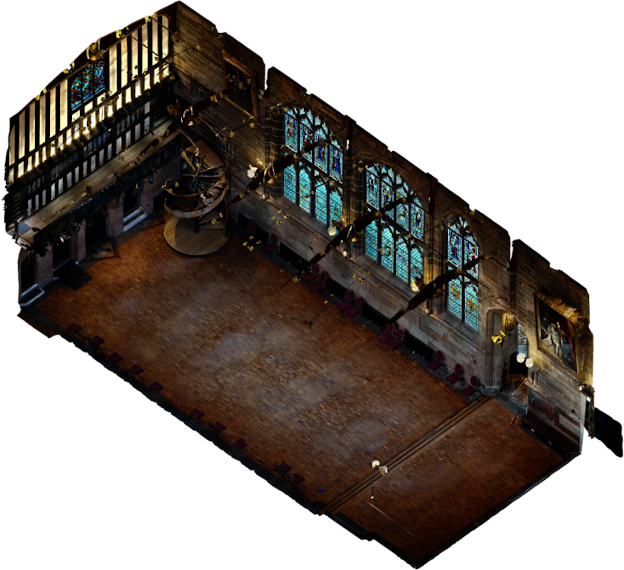
\includegraphics[width=0.7\linewidth]{guildhall}
    \caption[Proof of concept demonstration --- large environment]{St Mary's Guildhall: a Medieval-style church in Coventry, West Midlands, England. The large environment has a unique soundscape, characterised by a recorded $T_{60}$ reverberation time of over a second.}
    \label{fig:guildhall-iso-render}
\end{figure}

\begin{figure}[htbp]
    \centering
    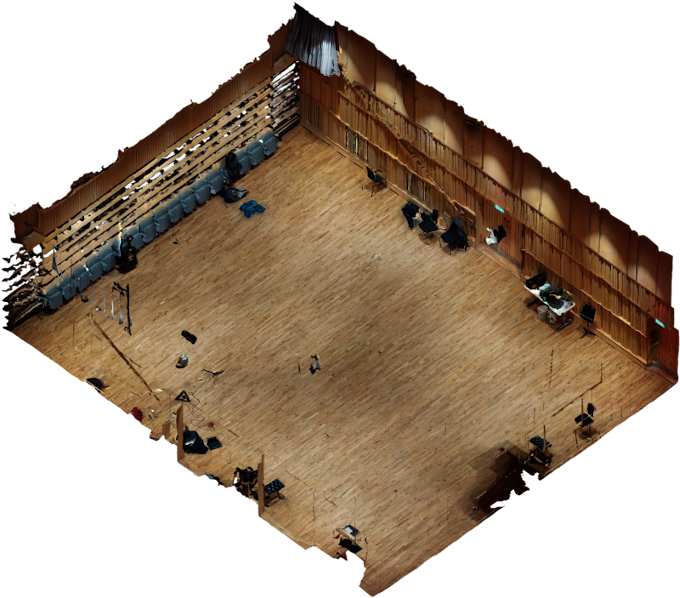
\includegraphics[width=0.7\linewidth]{recital-hall}
    \caption[Proof of concept demonstration --- medium environment]{Recital Hall: a wooden space serving as a stage for musical performances. The soundscape is characterised by a recorded $T_{60}$ reverberation time within a second.}
    \label{fig:conservatoire-iso-render}
\end{figure}

\begin{figure}[htbp]
    \centering
    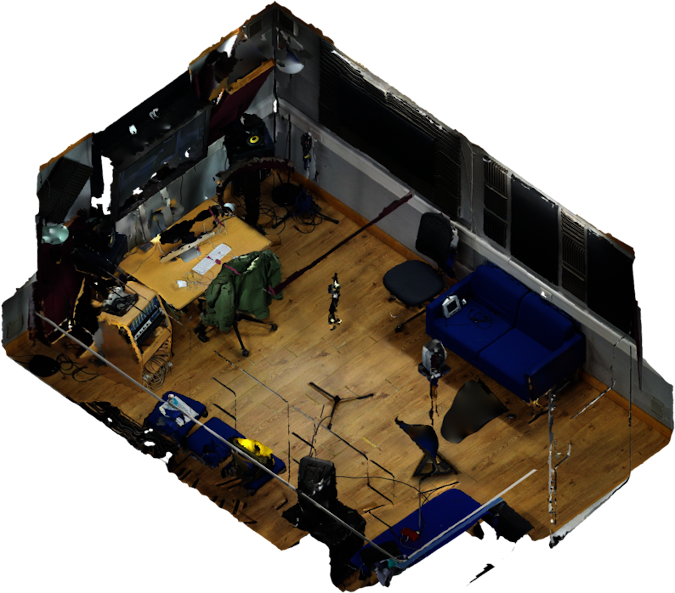
\includegraphics[width=0.7\linewidth]{mastering_suite}
    \caption[Proof of concept demonstration --- small environment]{Mastering Suite: a small audio production studio with acoustic treatments to minimise the effect of the soundscape on the sound reproduction system within.}
    \label{fig:mastering-iso-render}
\end{figure}

\section{Demonstration of Material Tagging on Real Data}
%Mastering Suite
\begin{figure}
    \centering
    \begin{subfigure}[t]{0.3\textwidth}
       \centering
       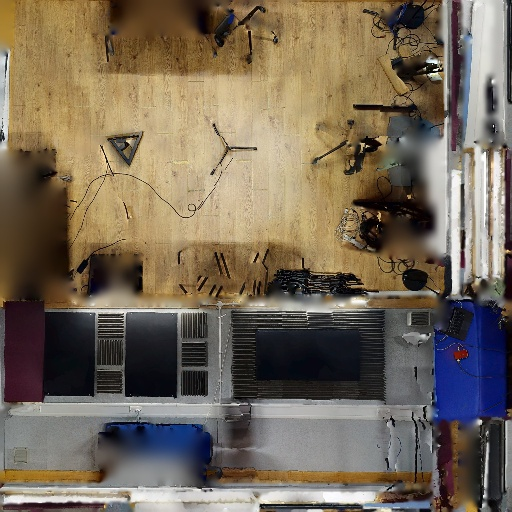
\includegraphics[width=\textwidth]{poc/t_mastering_suite_0.jpg}

    \end{subfigure}
    \begin{subfigure}[t]{0.3\textwidth}
       \centering
       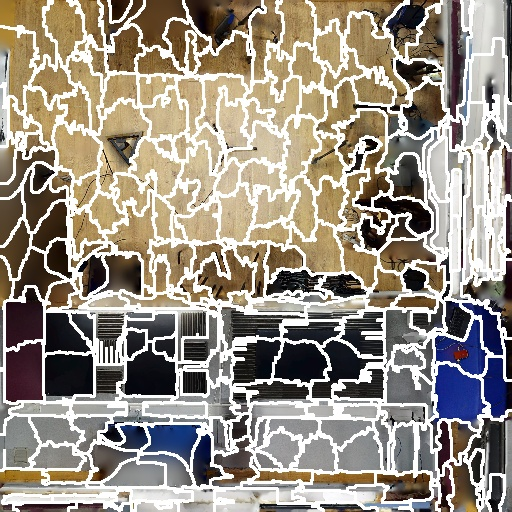
\includegraphics[width=\textwidth]{poc/x_mastering_suite_0.jpg}

    \end{subfigure}
    \begin{subfigure}[t]{0.3\textwidth}
        \centering
        
\includegraphics[width=\textwidth]{poc/s_mastering_suite_0.jpg}
     \end{subfigure}


    \addvspace{\baselineskip}


    \centering
    \begin{subfigure}[t]{0.3\textwidth}
       \centering
       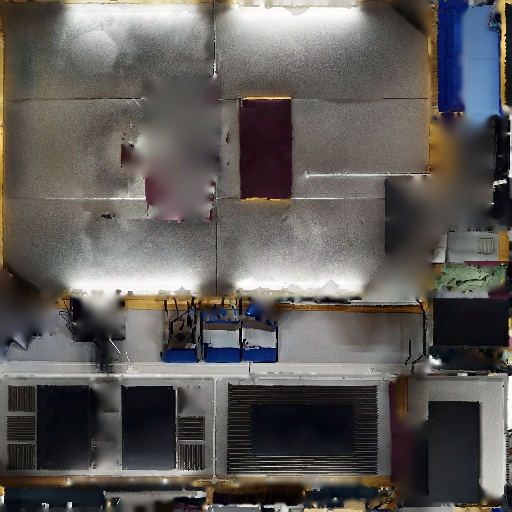
\includegraphics[width=\textwidth]{poc/t_mastering_suite_1.jpg}

    \end{subfigure}
    \begin{subfigure}[t]{0.3\textwidth}
       \centering
       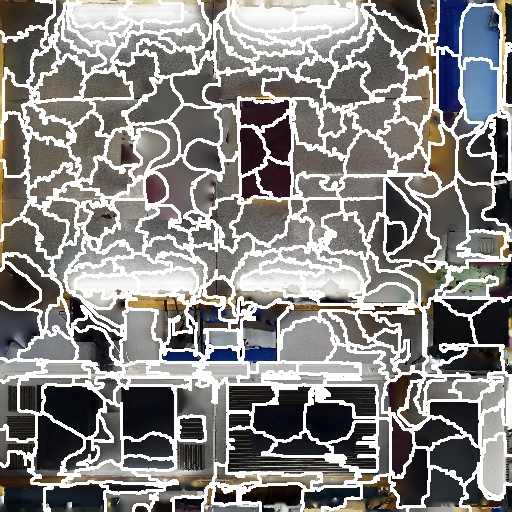
\includegraphics[width=\textwidth]{poc/x_mastering_suite_1.jpg}

    \end{subfigure}
    \begin{subfigure}[t]{0.3\textwidth}
        \centering
        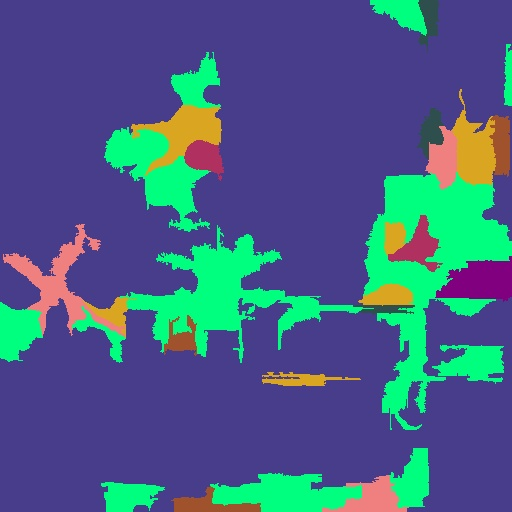
\includegraphics[width=\textwidth]{poc/s_mastering_suite_1.jpg}
     \end{subfigure}


    \addvspace{\baselineskip}

    
    \centering
    \begin{subfigure}[t]{0.3\textwidth}
       \centering
       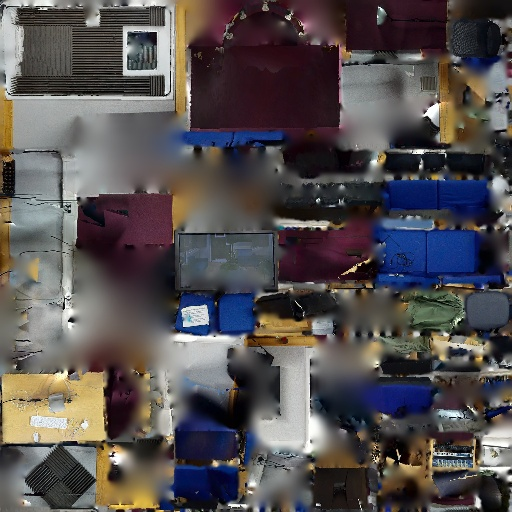
\includegraphics[width=\textwidth]{poc/t_mastering_suite_2.jpg}
       \caption{Input Texture}
    \end{subfigure}
    \begin{subfigure}[t]{0.3\textwidth}
       \centering
       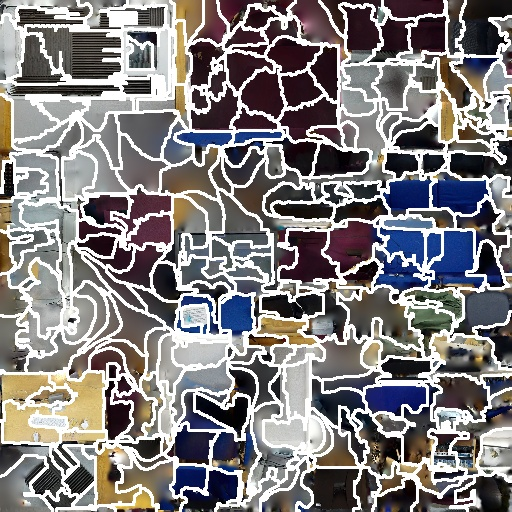
\includegraphics[width=\textwidth]{poc/x_mastering_suite_2.jpg}
       \caption{Superpixel Segmentation}
    \end{subfigure}
    \begin{subfigure}[t]{0.3\textwidth}
        \centering
        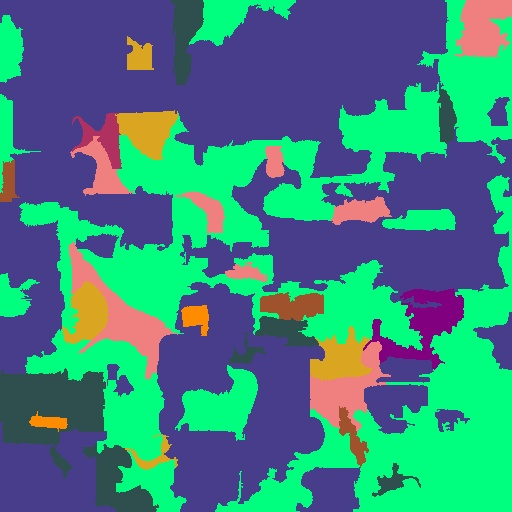
\includegraphics[width=\textwidth]{poc/s_mastering_suite_2.jpg}
        \caption{Material Tagging}
     \end{subfigure}
 

\caption{Material Tagging performed on textures from the Mastering Suite scene.}
\label{fig:mastering-suite-superpixels}
\end{figure}
%Recital Hall
\begin{figure}
    \centering
    \begin{subfigure}[t]{0.3\textwidth}
       \centering
       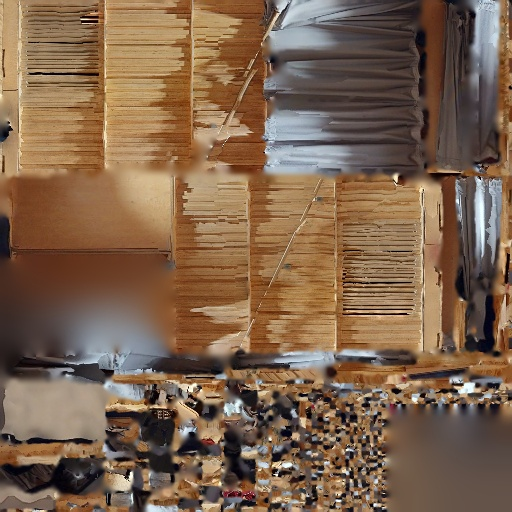
\includegraphics[width=\textwidth]{poc/t_conservatoire_0.jpg}

    \end{subfigure}
    \begin{subfigure}[t]{0.3\textwidth}
       \centering
       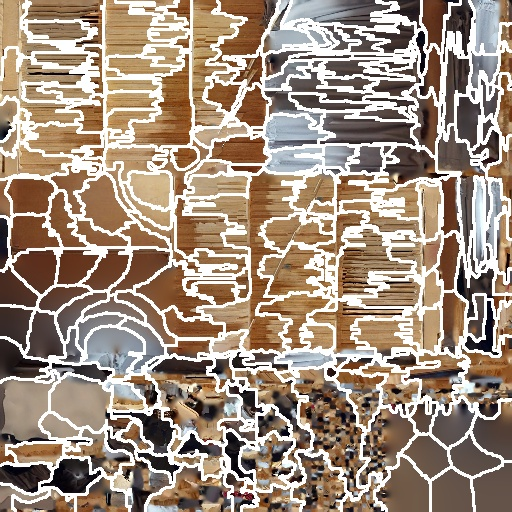
\includegraphics[width=\textwidth]{poc/x_conservatoire_0.jpg}

    \end{subfigure}
    \begin{subfigure}[t]{0.3\textwidth}
        \centering
        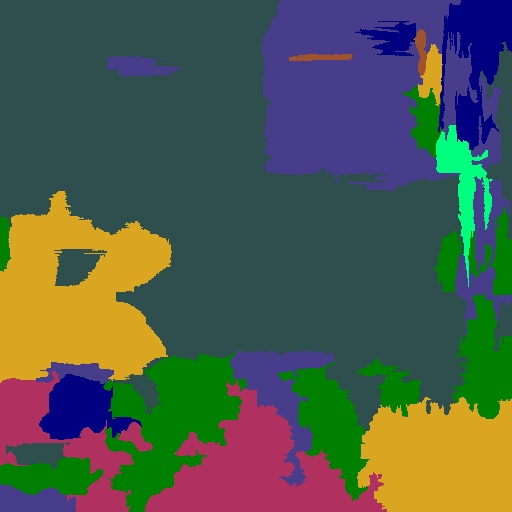
\includegraphics[width=\textwidth]{poc/s_conservatoire_0.jpg}
     \end{subfigure}


    \addvspace{\baselineskip}


    \centering
    \begin{subfigure}[t]{0.3\textwidth}
       \centering
       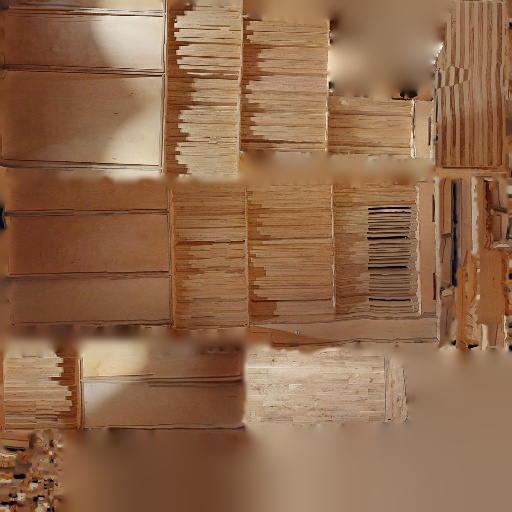
\includegraphics[width=\textwidth]{poc/t_conservatoire_1.jpg}

    \end{subfigure}
    \begin{subfigure}[t]{0.3\textwidth}
       \centering
       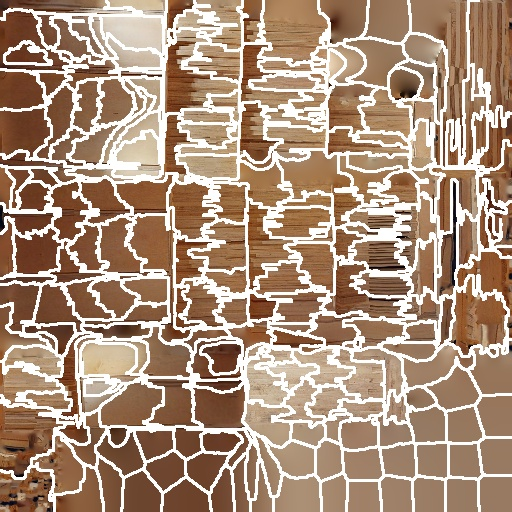
\includegraphics[width=\textwidth]{poc/x_conservatoire_1.jpg}

    \end{subfigure}
    \begin{subfigure}[t]{0.3\textwidth}
        \centering
        
\includegraphics[width=\textwidth]{poc/s_conservatoire_1.jpg}
     \end{subfigure}


    \addvspace{\baselineskip}

    
    \centering
    \begin{subfigure}[t]{0.3\textwidth}
       \centering
       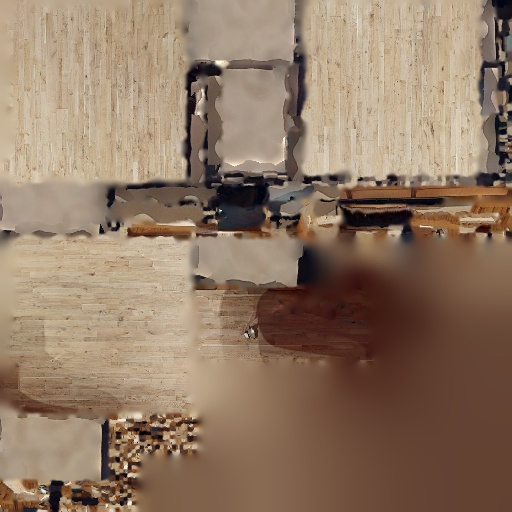
\includegraphics[width=\textwidth]{poc/t_conservatoire_2.jpg}
       \caption{Input Texture}
    \end{subfigure}
    \begin{subfigure}[t]{0.3\textwidth}
       \centering
       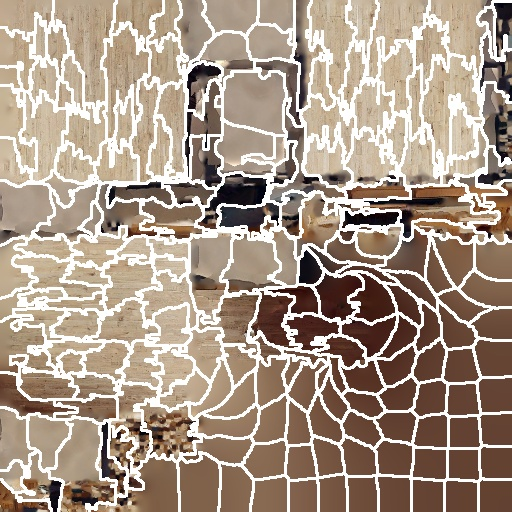
\includegraphics[width=\textwidth]{poc/x_conservatoire_2.jpg}
       \caption{Superpixel Segmentation}
    \end{subfigure}
    \begin{subfigure}[t]{0.3\textwidth}
        \centering
        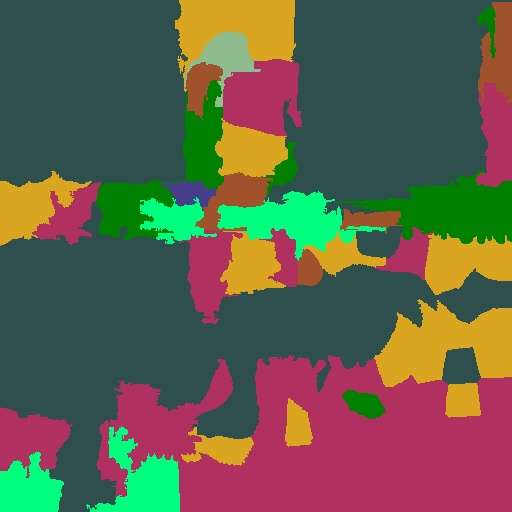
\includegraphics[width=\textwidth]{poc/s_conservatoire_2.jpg}
        \caption{Material Tagging}
     \end{subfigure}
 

\caption{Material Tagging performed on textures from the Recital Hall scene.}
\label{fig:recital-hall-superpixels}
\end{figure}
%Guild Hall
\begin{figure}
    \centering
    \begin{subfigure}[t]{0.3\textwidth}
       \centering
       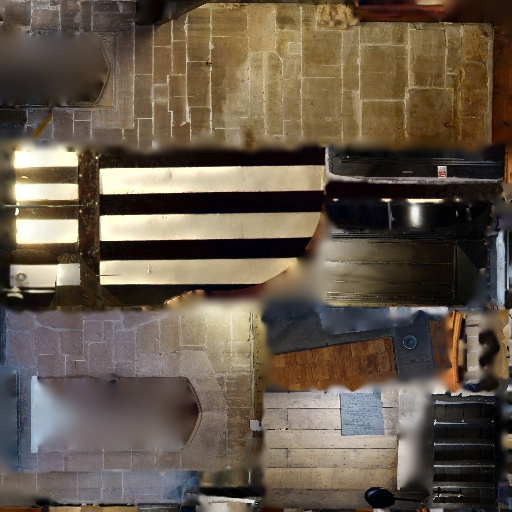
\includegraphics[width=\textwidth]{poc/t_GuildHall_0.jpg}

    \end{subfigure}
    \begin{subfigure}[t]{0.3\textwidth}
       \centering
       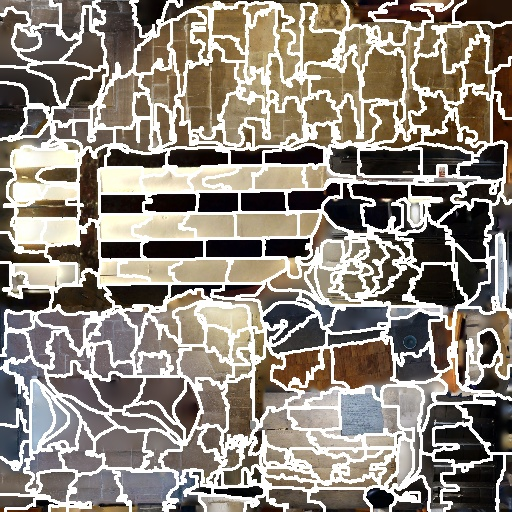
\includegraphics[width=\textwidth]{poc/x_GuildHall_0.jpg}

    \end{subfigure}
    \begin{subfigure}[t]{0.3\textwidth}
        \centering
        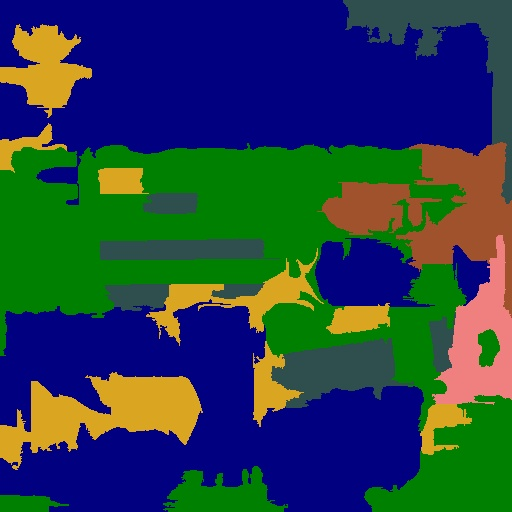
\includegraphics[width=\textwidth]{poc/s_GuildHall_0.jpg}
     \end{subfigure}


    \addvspace{\baselineskip}


    \centering
    \begin{subfigure}[t]{0.3\textwidth}
       \centering
       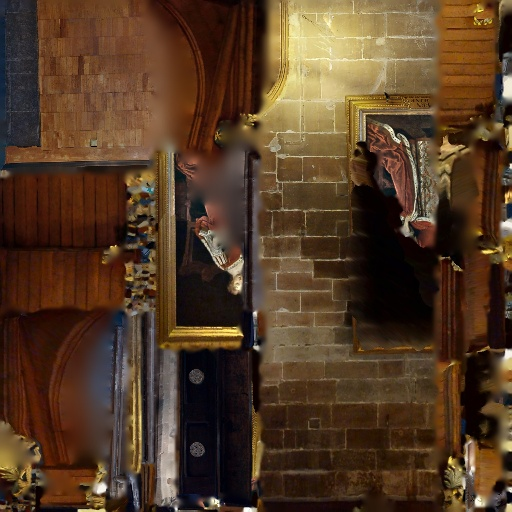
\includegraphics[width=\textwidth]{poc/t_GuildHall_1.jpg}

    \end{subfigure}
    \begin{subfigure}[t]{0.3\textwidth}
       \centering
       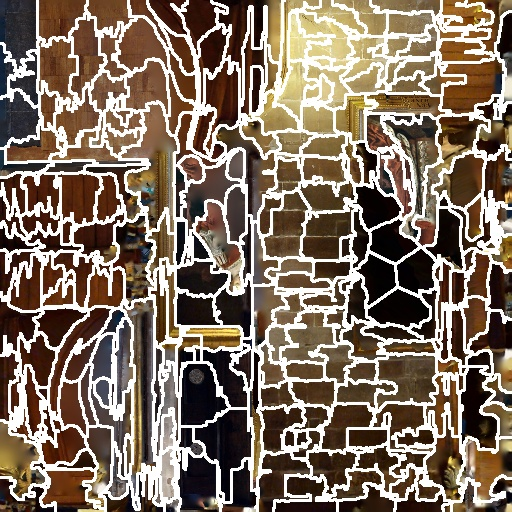
\includegraphics[width=\textwidth]{poc/x_GuildHall_1.jpg}

    \end{subfigure}
    \begin{subfigure}[t]{0.3\textwidth}
        \centering
        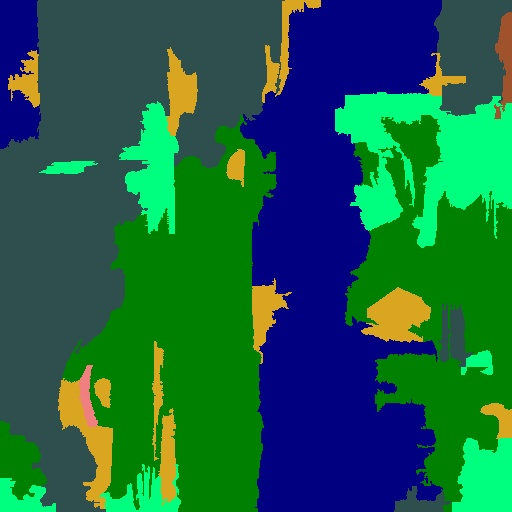
\includegraphics[width=\textwidth]{poc/s_GuildHall_1.jpg}
     \end{subfigure}


    \addvspace{\baselineskip}

    
    \centering
    \begin{subfigure}[t]{0.3\textwidth}
       \centering
       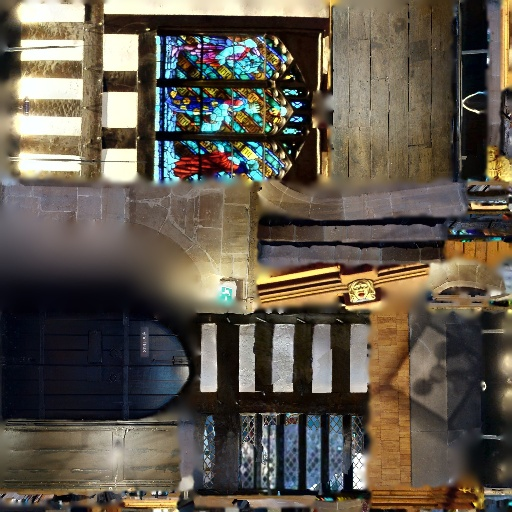
\includegraphics[width=\textwidth]{poc/t_GuildHall_2.jpg}
       \caption{Input Texture}
    \end{subfigure}
    \begin{subfigure}[t]{0.3\textwidth}
       \centering
       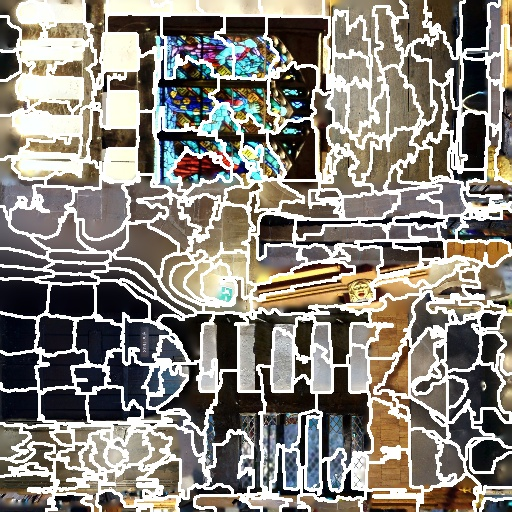
\includegraphics[width=\textwidth]{poc/x_GuildHall_2.jpg}
       \caption{Superpixel Segmentation}
    \end{subfigure}
    \begin{subfigure}[t]{0.3\textwidth}
        \centering
        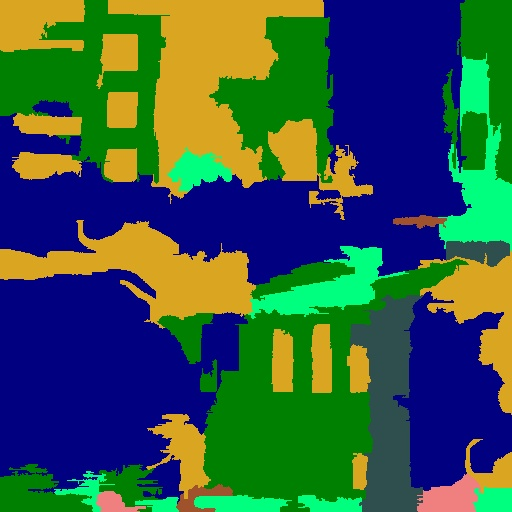
\includegraphics[width=\textwidth]{poc/s_GuildHall_2.jpg}
        \caption{Material Tagging}
     \end{subfigure}
 

\caption{Material Tagging performed on textures from the St Mary's Guild Hall scene.}
\label{fig:guild-hall-superpixels}
\end{figure}
